\section{Overview}
The PowerEnjoy system is designed as a 3-tier application:
\begin{itemize}
\item \textbf{Data tier:} A PostgreSQL DB, deployed on AWS and replicated for availability and integrity. 
\item \textbf{Application tier:} A NodeJS application that provides APIs, deployed on AWS and replicated. The Express library is used to realise API endpoints. These APIs are exposed in a REST manner, responses are JSONs. The replication of the application grants fault tolerance and, using a load balancer, also availability.
\item \textbf{Presentation tier:} The presentation layer is realised with the 2 mobile applications (Driver and Worker), the web portal (Driver) and the Administrator application. The web portal is realised using EJS templating (server-side) and JQuery (client-side).
\end{itemize}
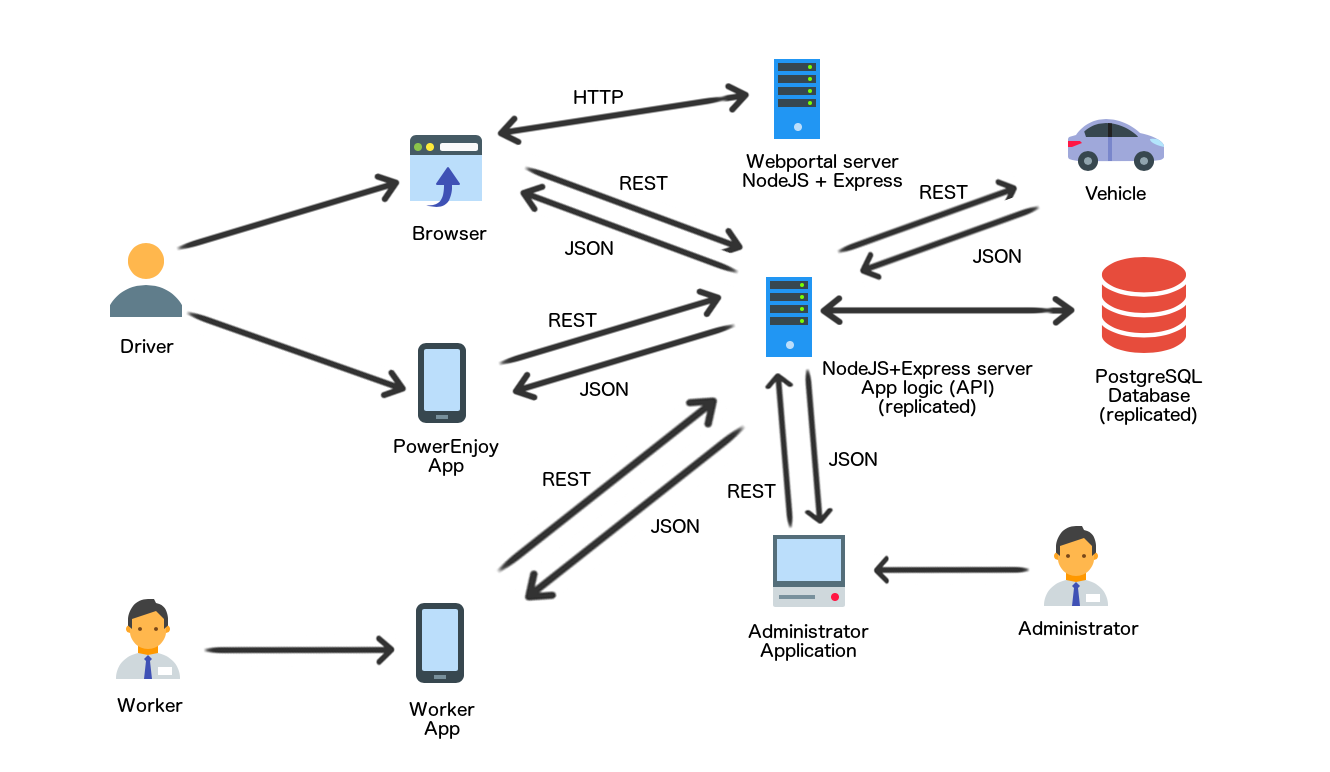
\includegraphics[width=13cm,keepaspectratio]{archi}

\section{High level components}
The high level structure of the System can be divided into X components. The main component is the \textbf{core}, that receives requests from \textbf{clients}, either \textbf{drivers}, \textbf{workers} and \textbf{administrators}; depending on the client type, the component provides different interfaces. 
The core also communicates with the \textbf{DBMS} component, responsible of data persistence. 
The core implements all the business logic: 
\begin{itemize}
\item Process drivers requests and allocates the requested vehicle 
\item Manages vehicles, track their state
\item Manages users (drivers signup, login)
\item Manages reports and automatic tasks then it allocates them to workers
\end{itemize}